\section{A positive arithmetic counting boundary}
\label{sec:positive-arithmetic-reference}

A nontrivial arithmetic boundary can retain the actual field operations
while changing the reference preparation. The construction here assigns
positive mass to each absolute Frobenius period and matches the ordinary
maximally mixed state at the actual characteristic. Its unnormalized density
has positive Taylor coefficients; its normalized state is a Poisson mixture. Its boundary requires only a finite operator polynomial for
every finite reference experiment. This polynomial preserves the leading
probability and conditional state of every later arithmetic branch, including
coherent mixed circuits. The characteristic and field tables remain named
data. The six positive statements below have passed the capped review.

\subsection{The reference and its positive coefficients}

For a fixed actual prime $p$ and named primitive root $\zeta_p$, an
arithmetic field $E=\mathbb F_{p^r}$ has register $H_E=\ell^2(E)$,
orthonormal basis $|x\rangle$, and character
$\psi_E(x)=\zeta_p^{\sum_{j=0}^{r-1}x^{p^j}}$. We use the actual matrices
\[
 U_E|x\rangle=|x^p\rangle,\qquad
 F_E|x\rangle=|E|^{-1/2}\sum_y\psi_E(-xy)|y\rangle,
\]
and, for a named embedding $i:K\to E$, $|K|=p^s$, $r=ns$,
\[
 T_i(y)=i^{-1}\!\left(\sum_{j=0}^{n-1}y^{p^{sj}}\right),\quad
 \kappa_i=|E|/|K|,\quad J_i|a\rangle=|i(a)\rangle,\quad
 V_i|a\rangle=\kappa_i^{-1/2}\sum_{T_i(y)=a}|y\rangle.
\]
The inverse embedding is restricted to its image and every square root is
positive. Both transfers are isometries, compose in named towers, and obey
$F_EJ_i=V_iF_K$ and $F_EV_i=J_iF_K$ in every characteristic.
Independent register lists use ordered tensor products.
\provenance{D1301--D1304, D1306, FRB-TRACE, FRB-TRANSFER}
{foundation.md; transfers-example.md}{arithmetic Frobenius checker}
{frobenius-hierarchy-adjudication.md}

\begin{definition}[Period-uniform arithmetic reference]
Fix the actual $p,\zeta_p$ and a finite diagram of named arithmetic fields
and embeddings. Let $h\geq0$ and $t=e^h$; the prime $p$ is retained data.
For $E=\mathbb F_{p^r}$ set $P_{E,0}=|0\rangle\langle0|$ and let
$P_{E,d}^{\times}$ project onto the nonzero labels of exact absolute
Frobenius period $d$, for $d\mid r$. Define
\[
 b_1(t)=t-1,\qquad b_d(t)=\sum_{e\mid d}\mu(d/e)t^e\quad(d>1),
\]
where $\mu$ is zero on integers divisible by a prime square and otherwise
is $(-1)$ to the number of distinct prime factors. Put
\[
 D_E(h)=P_{E,0}+\sum_{d\mid r}\frac{b_d(e^h)}{b_d(p)}P_{E,d}^{\times},
 \qquad \rho_E(h)=e^{-rh}D_E(h).
\]
A period-uniform density lies in the real span of these orthogonal
projections, without off-diagonal blocks. Its prescribed masses are
$e^{-rh}$ at zero and $e^{-rh}b_d(e^h)$ on the nonzero period blocks.
For an ordered word $E_1,\ldots,E_m$ use tensor products $D_{\rm word}$
and $\rho_{\rm word}$, and put $R=\sum_jr_j$. The empty word has
$D=\rho=1$ and $R=0$. This reference is additional preparation data.
\end{definition}
\begin{scope}
The actual maximally mixed preparation remains its original constant
arithmetic map. The new reference varies a state, not a field cardinality
or the matrices of the arithmetic gates.
\end{scope}
\provenance{D1501}{definitions.md}{positive arithmetic checker P1}{positive-arithmetic-adjudication.md}

\begin{definition}[Positive reference coefficients]
Let $A_{E,0}=P_{E,0}$ and, for $k\geq1$, define
\begin{align*}
 J_k(d)&=\sum_{e\mid d}\mu(d/e)e^k
       =d^k\prod_{\ell\mid d\,\mathrm{prime}}(1-\ell^{-k}),\\
 A_{E,k}&=\sum_{d\mid r}\frac{J_k(d)}{k!b_d(p)}P_{E,d}^{\times},
 \qquad B_E=A_{E,1}.
\end{align*}
The empty product gives $J_k(1)=1$. Set $\sigma_{E,0}=P_{E,0}$ and
$\sigma_{E,k}=k!A_{E,k}/r^k$ for $k\geq1$. Word coefficients are
\[
 A_{{\rm word},k}=\sum_{k_1+\cdots+k_m=k}\bigotimes_j A_{E_j,k_j}.
\]
For nonempty words define $\sigma_{{\rm word},k}=k!A_{{\rm word},k}/R^k$
when $k\geq1$, and use the all-zero projection at grade zero.
\end{definition}
\begin{scope}
These grades refer to powers of $h$, not to a Clifford hierarchy level.
The full positive series will have a separate finite sufficient profile.
\end{scope}
\provenance{D1502}{definitions.md}{positive arithmetic checker P1, P5}{positive-arithmetic-adjudication.md}

\begin{proposition}[A unique positive reference and its Poisson decomposition]
\statusProved\quad
For every actual finite field $E=\mathbb F_{p^r}$, $\rho_E(h)$ is the
unique period-uniform state with the prescribed masses. It is faithful for
$h>0$, equals $I/p^r$ exactly at $h=\log p$, and tends to $P_{E,0}$ at zero.
The unnormalized density has the entire trace-norm convergent expansion
\[
 D_E(h)=\sum_{k\geq0}h^kA_{E,k},\qquad
 \operatorname{Tr}A_{E,k}=\frac{r^k}{k!},\qquad
 \rho_E(h)=e^{-rh}\sum_{k\geq0}\frac{(rh)^k}{k!}\sigma_{E,k}.
\]
For $k\geq1$, $A_{E,k}$ is positive definite on the nonzero-label subspace.
On a nonempty independent word,
\[
 \sigma_{{\rm word},k}=
 \sum_{k_1+\cdots+k_m=k}
 \frac{k!}{\prod_jk_j!}\prod_j\left(\frac{r_j}{R}\right)^{k_j}
 \bigotimes_j\sigma_{E_j,k_j}.
\]
Thus grades compose with multinomial weights, binomial for two factors.
On the full matrix algebra the reference is tracial only at $h=\log p$.
\end{proposition}
\begin{scope}
The coefficient states and register dimensions retain $p$. Uniqueness
uses the explicitly stated scalar action on each period block, not only
agreement of the diagonal entries of an otherwise arbitrary density.
\end{scope}
\provenance{POS-STATE}{reference-and-protocol.md, Sections 1--2}
{positive arithmetic checker P1, P7}{positive-arithmetic-adjudication.md}

\begin{proof}[Derivation]
Expanding the divisor sum for $b_d(e^h)$ gives
$\sum_{k\geq1}h^kJ_k(d)/k!$, including $d=1$. Every $J_k(d)$ is positive
by its prime-factor product, and $\sum_{d\mid r}J_k(d)=r^k$ by cancellation
of the inner Moebius divisor sum. The nonzero period block has rank $b_d(p)$,
so the displayed trace formulas follow. The masses fix the scalar on
each block uniquely. Comparing the zero and one basis entries shows that
their commutator test vanishes only when $e^h=p$, where the density is
indeed scalar. Independent multiplication of the convergent series gives
the multinomial weights.
\end{proof}

\begin{definition}[Finite positive reference profile]
Put
\[
 L_E(h)=P_{E,0}+hB_E,\qquad
 L_{\rm word}(h)=\bigotimes_jL_{E_j}(h),\qquad
 \lambda_{\rm word}(h)=\frac{L_{\rm word}(h)}{\operatorname{Tr}L_{\rm word}(h)}.
\]
A positive operator polynomial is a finite sum $A(h)=\sum_{k=0}^mh^kA_k$
with every coefficient positive in its finite block matrix algebra; zero
coefficients are retained. For a subset $S$ of word positions define
\[
 P_S=\bigotimes_j\begin{cases}I-P_{E_j,0}&j\in S,\\P_{E_j,0}&j\notin S,
 \end{cases}\qquad
 B_S=\bigotimes_j\begin{cases}B_{E_j}&j\in S,\\P_{E_j,0}&j\notin S.
 \end{cases}
\]
Then $L_{\rm word}=\sum_Sh^{|S|}B_S$ and
$\operatorname{Tr}L_{\rm word}=\prod_j(1+r_jh)$.
\end{definition}
\begin{scope}
$D$ and $L$ are different families. The finite profile retains all data
needed for the leading operational questions proved below, rather than
all subleading probabilities at finite $h$.
\end{scope}
\provenance{D1503}{definitions.md}{positive arithmetic checker P5}{positive-arithmetic-adjudication.md}

\subsection{All named embeddings and arithmetic counting diagnostics}

\begin{proposition}[Reference restriction through every finite-field tower]
\statusProved\quad
For every named embedding $i:K\to E$, with absolute degrees $s,r$, in
every characteristic and relative degree,
\[
 J_i^*D_E(h)J_i=D_K(h),\qquad J_i^*A_{E,k}J_i=A_{K,k},\qquad
 J_i^*L_E(h)J_i=L_K(h).
\]
The retained inclusion decoder on $\rho_E(h)$ succeeds with probability
$e^{(s-r)h}$ and returns $\rho_K(h)$ on success. These restrictions and
successful probabilities compose exactly in all named towers.
For the transported reference $F_E\rho_E(h)F_E^*$, the retained $V_i$
decoder has the same success probability and returns
$F_K\rho_K(h)F_K^*$. Its failure output is also the Fourier transport of
the corresponding inclusion-decoder failure. Frobenius commutes with each
reference coefficient. For $\lambda_E$ the inclusion success probability
is $(1+sh)/(1+rh)$ and the conditional output is $\lambda_K$.
\end{proposition}
\begin{scope}
No inverse relative degree is used. Canonical references are natural under
named field embeddings and isomorphisms, not under arbitrary Hilbert-space
coordinate identifications. Fourier transports a reference to its actual
conjugate, which need not equal the canonical reference.
\end{scope}
\provenance{POS-DIAGRAM}{reference-and-protocol.md, Section 3}
{positive arithmetic checker P2, P3}{positive-arithmetic-adjudication.md}

\begin{proof}[Derivation]
An embedding preserves and reflects $x^{p^d}=x$ by injectivity, so it
preserves exact absolute Frobenius period and zero. The coefficient attached
to a period uses $b_d(p)$ independently of the ambient field, proving all
three restrictions. Trace normalization gives the success probability.
The Fourier transfer identity gives the success square, while
$(I-V_iV_i^*)F_E=F_E(I-J_iJ_i^*)$ gives the failure square.
\end{proof}

\begin{proposition}[Frobenius moments and active multiplication mass]
\statusProved\quad
For every finite field $E=\mathbb F_{p^r}$ and integer $k$,
\[
 \operatorname{Tr}(\rho_E(h)U_E^k)=e^{(\gcd(r,k)-r)h},
 \qquad \gcd(r,0)=r.
\]
On $d\geq1$ independently prepared E controls and one E target, use the
actual multiplication gate
\[
 M|x_1,\ldots,x_d,z\rangle=|x_1,\ldots,x_d,z+\textstyle\prod_jx_j\rangle.
\]
The probability of all controls being
nonzero, its gate trace, and squared-difference expectation are
\begin{gather*}
 w_d(h)=(1-e^{-rh})^d,\qquad
 \operatorname{Tr}(\rho_E(h)^{\otimes(d+1)}M)=1-w_d(h),\\
 \operatorname{Tr}(\rho_E(h)^{\otimes(d+1)}(M-I)^*(M-I))=2w_d(h).
\end{gather*}
The active mass has order $d$ with leading coefficient $r^d$.
For $r\geq2$, conditioning on nonfixed Frobenius basis labels and
restricting to the marked common matrix action on every length-$d$ orbit
gives weights
\[
 \frac{b_d(e^h)}{e^{rh}-e^h}\longrightarrow\frac{\varphi(d)}{r-1},
 \qquad d\mid r,\ d>1,
\]
with normalized block trace $\operatorname{Tr}/d$. Here
$\varphi(d)=J_1(d)$ counts integers from one through d coprime to d.
\end{proposition}
\begin{scope}
These are specified reference expectations, not a tracial-state assertion
or a rule obtained by continuing every coupled arithmetic point count.
At $r=1$ the moving-label conditional sector is absent.
\end{scope}
\provenance{POS-COUNTS}{reference-and-protocol.md, Section 4}
{positive arithmetic checker P1, P6}{positive-arithmetic-adjudication.md}

The first formula sums precisely the period blocks fixed by the given
power. Multiplication fixes a basis tuple precisely when a control is zero;
the product reference is diagonal, so the same fixed-label test computes
its trace. This uses no translation invariance of the target state.
On an orbit block, the scalar reference coefficient cancels the actual
number of orbits, giving the stated conditional moving-orbit trace.

\subsection{Processes, profiles and conditional boundary records}

\begin{definition}[Positive-series process category]
Objects are finite tagged direct sums of matrix algebras, with trace the
sum of their ordinary matrix traces. A scalar normalizer is
$Z(h)=\sum_{k\geq0}z_kh^k$ with $z_k\geq0$, $z_0>0$, and finite value
for every real $h\geq0$. A process representative $X\to Y$ is
$(\Phi,Z)$ with $\Phi(h)=\sum_{k\geq0}h^k\Phi_k$, each $\Phi_k$ completely
positive, satisfying
\[
 \operatorname{Tr}_Y\Phi_k(a)\leq z_k\operatorname{Tr}_X(a)
 \quad\text{for every }a\geq0\text{ and every }k.
\]
It is normalized when equality holds throughout. Instruments retain their
external output tags. Equality is $Z'\Phi=Z\Phi'$ coefficientwise with
identical tags. Composition and tensor use Cauchy products and multiply
normalizers; the identity is $(\mathrm{id},1)$. Evaluation is $\Phi(h)/Z(h)$.
\end{definition}
\begin{scope}
This is a semantic CP category, with ordinary trace normalization. It does
not assert a faithful encoding of distinct source Kraus presentations.
Leading normalized states are not the equality relation.
\end{scope}
\provenance{D1504}{definitions.md}{positive arithmetic checker P5}{positive-arithmetic-adjudication.md}

\begin{definition}[Arithmetic profile experiments and boundary records]
Retain every actual constant arithmetic CP process. Its action on a
positive polynomial is $\Phi_*A=\sum_kh^k\Phi(A_k)$.
A profile experiment object is $(X,A)$, and an arrow
$(X,A)\to(Y,C)$ is such a constant map with $C=\Phi_*A$; equality means
equality of its typed CP map. Identity, composition and tensor use the
actual matrix operations, with Cauchy tensor on profiles. Zero profiles
are allowed but have no conditional state. The explicitly larger envelope
may use all finite-dimensional constant CP maps.
A finite reference protocol is a finite circuit of actual constant
arithmetic maps and either $\rho_E$ or $\lambda_E$ preparations, with
finitely many reference registers, named measurement placement and retained
histories. Coherent amplitude compositions use the actual matrices before
any prescribed CP instrument is applied.
For a nonzero positive series $A(h)=\sum_kh^kA_k$, define
\[
 v(A)=\min\{k:A_k\ne0\},\quad M(A)=A_{v(A)},\quad
 w(A)=\operatorname{Tr}M(A),\quad \eta(A)=M(A)/w(A).
\]
The boundary record is $(v,M)$, equivalently $(v,w,\eta)$. With scalar
normalizer having constant term $z_0$, its event probability has leading
coefficient $w/z_0$, order $v$, and conditional limit $\eta$.
Conditioning divides by the actual positive branch trace. The full profile
is retained before later conditioning or continuation.
\end{definition}
\begin{scope}
Canonical reference profiles are marked preparation data, not objects
preserved by arbitrary arithmetic channels. Leading normalization alone
is not an arrow or a functor on conditioned experiments.
\end{scope}
\provenance{D1505, D1506}{definitions.md}{positive arithmetic checker P4, P5}{positive-arithmetic-adjudication.md}

\begin{proposition}[Positive composition with the full arithmetic source]
\statusProved\quad
The positive-series processes form a symmetric monoidal category with
continuous CP, ordinary-trace-nonincreasing evaluation for every $h\geq0$.
It contains every actual constant arithmetic CP map as $(\Phi,1)$ and the
normalized preparation representatives
\[
 (z\mapsto zD_E(h),e^{rh}),\qquad (z\mapsto zL_E(h),1+rh).
\]
All actual amplitude equations and coherent arithmetic compositions retain
their original matrices. Profile experiments form a symmetric monoidal
category under coefficientwise CP action; all named instrument outcomes
and sequential histories can be retained.
\end{proposition}
\begin{scope}
The broader series category allows additional positive-series processes.
The finite sufficient profile theorem below concerns fixed CP branches
and finite protocols generated by the stated reference preparations and
constant arithmetic processes. The two scopes are distinct.
\end{scope}
\provenance{POS-PROCESS}{finite-operational-boundary.md, Sections 1--3}
{positive arithmetic checker P4, P5}{positive-arithmetic-adjudication.md}

Positive coefficients remain CP under Cauchy composition and tensor.
Their ordinary trace bounds multiply with the scalar normalizers and bound
all matrix-entry series on compact intervals. Cross-multiplied equality
respects composition because scalar series commute with the maps and a
scalar series with nonzero constant term can be cancelled coefficientwise.
The reference preparations satisfy coefficient normalization because
$\operatorname{Tr}A_{E,k}=r^k/k!$.

\begin{proposition}[A finite sufficient profile for every future CP branch]
\statusProved\quad
Let $E_1,\ldots,E_m$ be any finite reference word and let $\Phi$ be any
nonzero fixed finite-dimensional CP map on its full register. Then
$\Phi(D_{\rm word})$ and $\Phi(L_{\rm word})$ have the same first nonzero
matrix coefficient and the same vanishing order, at most $m$.
The conclusion remains valid after arbitrary later fixed CP continuation
and independent tensor, including entangling maps.
Consequently every finite reference protocol has identical leading event
orders, probability coefficients and conditional output densities under
the exact and finite-profile preparations. Keeping the full polynomial
suffices for every such future branch question.
\end{proposition}
\begin{scope}
Subleading probabilities and entire finite-$h$ families are not asserted
equal. The degree bound counts all reference registers allocated to a
finite protocol, including those reserved for alternative adaptive histories.
The zero branch has no conditional limit under either preparation.
\end{scope}
\provenance{POS-FINITE}{finite-operational-boundary.md, Sections 4--6}
{positive arithmetic checker P5}{positive-arithmetic-adjudication.md}

\begin{proof}[Derivation]
On each nonzero support mask $S$, the exact word begins as
$h^{|S|}B_S$ and has only positive higher coefficients supported on that
mask. The matrix $B_S$ is positive definite there. If $\Phi(B_S)=0$,
positivity forces $\Phi$ to annihilate every positive matrix on the mask:
such a matrix is bounded above by a scalar multiple of $B_S$. Linearity
then kills the whole supported algebra. Thus a killed mask contributes
no later coefficient. The first surviving mask size supplies precisely
the same leading sum $\sum_{|S|=v}\Phi(B_S)$ in the exact and polynomial
families. Some mask survives when $\Phi\ne0$, because $\sum_SB_S$ is
faithful on the full input space; hence $v\leq m$.
Any later branch is another fixed CP composite. A finite protocol may
allocate its independent reference inputs at the beginning and discard
those unused on a history, reducing every branch to this same argument.
Both word normalizers have constant term one, so their event coefficients
and normalized leading densities also agree.
\end{proof}

The retained finite grades have a direct probabilistic meaning. A factor
$\lambda_E$ is a mixture of $P_{E,0}$ and $B_E/r$ with activation
probability $rh/(1+rh)$. On a word, the grade-$k$ conditional mixture runs
over subsets $S$ of size $k$, with weights proportional to $\prod_{j\in S}r_j$.
The maximal grade $m$ is needed for the event that all reference labels
are nonzero. A leading state alone fails even on one field: it is $P_{E,0}$,
but a later nonzero-label test has a real order-one branch $hB_E$.

\subsection{One protocol detects the arithmetic operations together}

\begin{definition}[Relative-Frobenius multiplication protocol]
For a named proper embedding $i:K\to E$, let $q=p^s=|K|$ and choose
named $a,b\in E$ satisfying $T_i(ab)=0$ and $T_i(a^qb)=1$.
Prepare the reference word $E,E,K$, retaining the outcome selecting its
computational labels $a,b,0$. Apply $V_i$ to the target, $U_E^s$ to the
first control, the actual multiplication gate
\[
 M_E^{(2)}|x,y,z\rangle=|x,y,z+xy\rangle,
\]
and then $F_E$ to the target. Apply the retained $J_i$ decoder, whose
success amplitude is $J_i^*$ and failure amplitude is $I-J_iJ_i^*$.
On success apply $F_K^*$ and measure the target label. All failures remain
tagged. An optional coherence test dephases the target in its E basis
immediately after $V_i$. Either exact or finite reference preparations
may be used, with their boundary records compared as above.
\end{definition}
\begin{scope}
The elements $a,b$ are named choices. Their existence for every proper
extension and the observable protocol outcomes are the following result.
\end{scope}
\provenance{D1507}{definitions.md}{positive arithmetic checker P4, P6}{positive-arithmetic-adjudication.md}

\begin{proposition}[A uniform mixed arithmetic boundary distinction]
\statusProved\quad
Every proper named finite-field embedding admits the choices $a,b$ above.
Its rare preparation has order two and positive leading coefficient
$w_aw_b$, where $w_x=\varphi(d)/b_d(p)$ for a nonzero label of period $d$.
The full protocol has decoder success one and final target $|1_K\rangle$.
Removing relative Frobenius or multiplication gives $|0_K\rangle$.
Removing target Fourier gives decoder success $1/\kappa_i$ when the
relative degree is invertible in $p$, and zero when it is divisible by $p$.
Dephasing the trace-fibre target changes decoder success from one to
$1/\kappa_i$, with final target still $|1_K\rangle$ on success.
For $\mathbb F_2\subset\mathbb F_4=\mathbb F_2[\alpha]/(\alpha^2+\alpha+1)$,
the choices $a=\alpha,b=\alpha^2$ have preparation coefficient $1/4$;
changing the multiplication entry $\alpha^2\alpha^2=\alpha$ to zero
changes the observed target from one to zero.
\end{proposition}
\begin{scope}
The result covers every proper finite extension, including
characteristic-dividing degrees. Output labels zero and one are uniform;
the preparation coefficient, matrices and dimensions retain characteristic
and field data. Coherent trace-fibre evolution is part of the experiment.
\end{scope}
\provenance{POS-MIXED}{reference-and-protocol.md, Section 5}
{positive arithmetic checker P4, P6, P7}{positive-arithmetic-adjudication.md}

\begin{proof}[Derivation]
Choose $a_0$ outside K. If $a_0,a_0^q$ are dependent, write
$a_0^q=\lambda a_0$ with $\lambda\ne1$ and use $a=a_0+1$; its two
coefficients in the independent pair $a_0,1$ show that $a,a^q$ are
independent. Otherwise use $a=a_0$. Nondegeneracy of the relative trace
pairing makes $b\mapsto(T_i(ab),T_i(a^qb))$ surjective onto $K^2$,
so the prescribed $b$ exists. Multiplication translates $V_i|0\rangle$
to $V_i|1\rangle$, and Fourier transports that to $J_iF_K|1\rangle$.
The decoder and final inverse Fourier therefore return one. Without
Frobenius or multiplication the same computation returns zero.
Without Fourier, the actual Gram column $J_i^*V_i|1\rangle$ has squared
norm $1/\kappa_i$ in the invertible-degree branch and vanishes in the
singular branch. A dephased trace fibre gives a mixture of basis vectors,
each with code success $1/\kappa_i$, which verifies the coherence test.
\end{proof}

\subsection{What the boundary retains}

For a concrete positivity comparison, take $\mathbb F_2\subset\mathbb F_8$.
The complement of the joint inclusion/trace-fibre code space has rank four
and kills the basis vectors $0,1$. Each of the six other labels has period
three and reference weight $(t^3-t)/(6t^3)$. Hence the new expectation of
this complementary projection is $\tfrac23(1-t^{-2})$, while the earlier
formal tracial prescription was $1-2t^{-2}$. Both agree with the actual
arithmetic trace at $t=2$. The positive extension uses a different reference
state, as illustrated in Figure~\ref{fig:positive-reference}.
\begin{figure}[htbp]
\centering
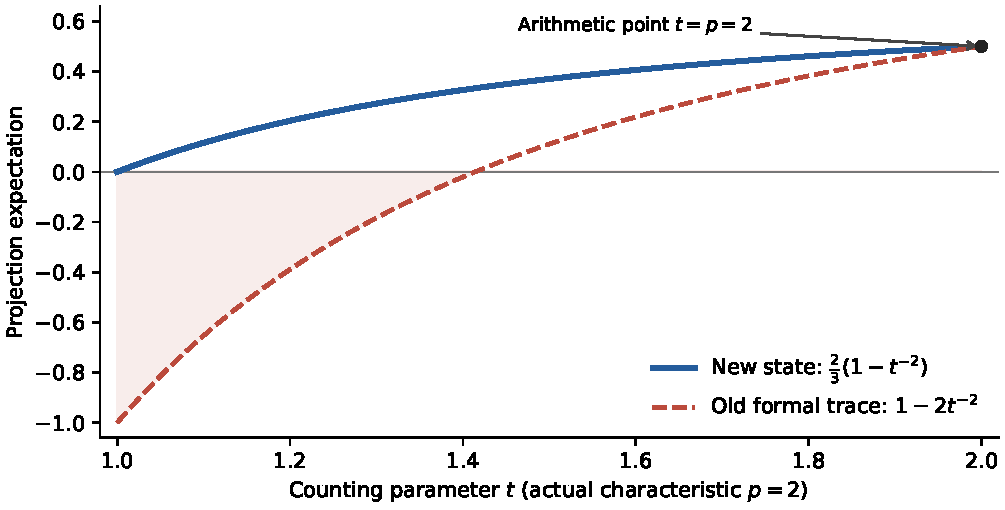
\includegraphics[width=0.88\linewidth]{figures/positive-arithmetic-reference.pdf}
\caption{A full positive state replaces the failed tracial continuation.
The arithmetic data are fixed at $\mathbb F_2\subset\mathbb F_8$; only
the counting reference varies. The shaded negative values cannot be
projection probabilities.}
\label{fig:positive-reference}
\end{figure}

The construction preserves actual arithmetic matrices and their relations,
and supplies a new positive normalization and finite operational rule.
One universal consequence is particularly simple. For a relative extension
$\mathbb F_{p^s}\subset\mathbb F_{p^{sn}}$, the first nonzero-sector
state satisfies, for every integer $j$,
\[
 \operatorname{Tr}\bigl(\sigma_{E,1}U_E^{sj}\bigr)
     =\frac{\gcd(n,j)}{n}.
\]
Indeed the coefficient of $h$ in
$\operatorname{Tr}(D_E(h)U_E^{sj})=e^{\gcd(sn,sj)h}$ is
$\operatorname{Tr}(B_EU_E^{sj})$, and $\sigma_{E,1}=B_E/(sn)$.
The relative Frobenius signature therefore depends only on the extension
degree. The full construction does not impose characteristic independence.
For a quadratic field,
the nonzero boundary state $B_E/2$ has Frobenius first moment $1/2$ for
both $p=2$ and $p=3$. At $p=2$ its basis weights are $1/2$ on the nonzero
prime-field label and $1/4$ on each other label; at $p=3$ they are $1/4$
on each nonzero prime-field label and $1/12$ on each of the six other labels.

Nor does this rule continue every coupled point count by substituting
$t$ for $p$. The event $x=y\ne0$ on two independently prepared E references
has probability $\sum_{x\ne0}\rho_E(x)^2$ and order two, consistently with
its containment in the event that both labels are nonzero. The actual copy
isometry $|x\rangle\mapsto|x,x\rangle$ transports one reference and gives
that event order one. Its output is correlated and is not reset to two
independent canonical references. Likewise a prime-field coordinate unitary
transports a field reference to its actual, generally correlated image.

The earlier two-chart continuation varies angle matrices. The present
construction keeps those actual matrices fixed and varies preparations.
Agreement with its normalized tangent or weighted tower connector is not
automatic. A comparison must specify its reference and channel maps and
prove the relevant diagrams. The concrete surviving content here is the
positive period normalization, a finite sufficient profile for every future
arithmetic branch, and the mixed zero-versus-one protocol above.
